\label{09-0221}
%%%%%%% Lecture Notes Style for Concrete Mathematics %%%%%%%%%%%%%
%%%%%%% Taught by Patrick White, TJHSST %%%%%%%%%%%%%%%%%%%%%%%%%%

% \documentclass[11pt,twosided]{article}
% %%%%%%%%%%%%%%%%%%%%%%%%%%%%%%%%%%%%%%%%%%%%%%%%%%%%%%%
%%%% HEADER FILE for CONCRETE MATH LECTURE NOTES %%%%%%
%%%%%%%%%%%%%%%%%%%%%%%%%%%%%%%%%%%%%%%%%%%%%%%%%%%%%%%

%%%%%%%%%%%%%%%%%%%%%%%%%%%%%%%%%%%%%%%%%%%%%%%%%%%%%%%%%%%%%%%%%%%
%% This file is included at the top of every lecture notes file %%%
%% It should ONLY be changed by the instructor %%
%%%%%%%%%%%%%%%%%%%%%%%%%%%%%%%%%%%%%%%%%%%%%%%%%%%%%%%%%%%%%%%%%%%

%%%%%%%%%%%%%%%%%%%%%% package inclusions %%%%%%%%%%%%%%%%%%%%
%\usepackage[
%top=2cm,
%bottom=2cm,
%left=3cm,
%right=2cm,
%headheight=17pt, % as per the warning by fancyhdr
%includehead,includefoot,
%heightrounded, % to avoid spurious underfull messages
%]{geometry} 


\usepackage{amsmath,amssymb,amsfonts}
\usepackage{longtable}
\usepackage{mathtools}
\usepackage{amsthm}
\usepackage{enumerate}
\usepackage{fancyhdr}
\pagestyle{fancy}


%%%%%%%%%%%%%%% theorem style definitions %%%%%%%%%%%%%%%%%%%%%%
\newtheorem{theorem}{Theorem}[section]
%\newtheorem{corollary}{Corollary}[theorem]
%\newtheorem{lemma}[theorem]{Lemma}
\newtheorem*{remark}{Remark}
%\newtheorem{example}{Example}[section]
\newtheorem*{definition}{Definition}


%%%%%%%%%%%%%%%% custom function definitions %%%%%%%%%%%%%%%%%%%%%%%%%
%%%%%%%%%%% as class progresses, this section may be enhanced %%%%%%%%

\def\multiset#1#2{\ensuremath{\left(\kern-.3em\left(\genfrac{}{}{0pt}{}{#1}{#2}\right)
		\kern-.3em\right)}} %%% multiset notation
\newcommand\rf[2]{{#1}^{\overline{#2}}} %%%% rising factorial \rf{x}{m}
\newcommand\ff[2]{{#1}^{\underline{#2}}} %%%%% falling factorial \ff{x}{m}
\newcommand{\Perm}[2]{{}^{#1}\!P_{#2}} % permutation
\newcommand{\half}{\ensuremath{\frac{1}{2}}}
\newcommand{\braces}[1]{\left\{#1\right\}}
\newcommand{\set}[1]{\braces{#1}}
\newcommand{\snb}[2]{\ensuremath{\left(\kern-.3em\left(\genfrac{}{}{0pt}{}{#1}{#2}\right)\kern-.3em\right)}}
\newcommand{\fallingfactorial}[1]{^{\underline{#1}}}
\newcommand{\fallfac}[2]{{#1}^{\underline{#2}}}
\newcommand{\stirlingone}[2]{\genfrac[]{0pt}{1}{#1}{#2}}
\newcommand{\stiri}[2]{\stirlingone{#1}{#2}}
\newcommand{\dstirlingone}[2]{\genfrac[]{0pt}{0}{#1}{#2}}
\newcommand{\dstiri}[2]{\dstirlingone{#1}{#2}}
\newcommand{\stirlingtwo}[2]{\genfrac\{\}{0pt}{1}{#1}{#2}}
\newcommand{\stirii}[2]{\stirlingtwo{#1}{#2}}
\newcommand{\dstirlingtwo}[2]{\genfrac\{\}{0pt}{0}{#1}{#2}}
\newcommand{\dstirii}[2]{\dstirlingtwo{#1}{#2}}
\newcommand{\ol}[1]{\overline{#1}}
%%%%%%%
% book stuff
%%%%%%%%%

\usepackage[twoside,outer=1.5in,inner=2in,bottom=1.5in,top=1.5in,marginpar=2in]{geometry} 
\usepackage{scrextend}
\usepackage{palatino}
\usepackage{multicol}
\usepackage{float}
\usepackage[hidelinks]{hyperref}
\usepackage[nameinlink, capitalise, noabbrev]{cleveref}
%\usepackage{background}
\usepackage{graphicx}
\usepackage{listliketab}

\usepackage{lipsum}
\usepackage{caption}
\usepackage{marginnote}

\reversemarginpar


\usepackage[dvipsnames]{xcolor}
\usepackage{amsthm}
\usepackage{shadethm}

\setlength{\parindent}{0pt}

\newcommand*\Note{%
	\marginnote[\textcolor{blue}{\raggedright{\LARGE ?}\ Note }]{}%
}
\newcommand*\Warn{%
	\marginnote[\textcolor{red}{\raggedright{\LARGE !}\ Warning }]{}%
}
\reversemarginpar

\newcommand{\N}{\mathbb{N}}
\newcommand{\Z}{\mathbb{Z}}
\newcommand{\I}{\mathbb{I}}
\newcommand{\R}{\mathbb{R}}
\newcommand{\Q}{\mathbb{Q}}
\renewcommand{\qed}{\hfill$\blacksquare$}
\let\newproof\proof
\renewenvironment{proof}{\begin{addmargin}[1em]{0em}\begin{newproof}}{\end{newproof}\end{addmargin}\qed}
% \newcommand{\expl}[1]{\text{\hfill[#1]}$}


\newenvironment{lemma}[2][Lemma]{\begin{trivlist}
		\item[\hskip \labelsep {\bfseries #1}\hskip \labelsep {\bfseries #2.}]}{\end{trivlist}}
\newenvironment{problem}[2][Problem]{\begin{trivlist}
		\item[\hskip \labelsep {\bfseries #1}\hskip \labelsep {\bfseries #2.}]}{\end{trivlist}}
\newenvironment{example}[2][Example]{\begin{trivlist}
		\item[\hskip \labelsep {\bfseries #1}\hskip \labelsep{\bfseries #2.}]}{\end{trivlist}}
\newenvironment{solution}{{\noindent \bfseries Solution\hskip 2ex}}{\qed}
\newenvironment{exercise}[2][Exercise]{\begin{trivlist}
		\item[\hskip \labelsep {\bfseries #1}\hskip \labelsep {\bfseries #2.}]}{\end{trivlist}}
\newenvironment{reflection}[2][Reflection]{\begin{trivlist}
		\item[\hskip \labelsep {\bfseries #1}\hskip \labelsep {\bfseries #2.}]}{\end{trivlist}}
\newenvironment{proposition}[2][Proposition]{\begin{trivlist}
		\item[\hskip \labelsep {\bfseries #1}\hskip \labelsep {\bfseries #2.}]}{\end{trivlist}}
\newenvironment{corollary}[2][Corollary]{\begin{trivlist}
		\item[\hskip \labelsep {\bfseries #1}\hskip \labelsep {\bfseries #2.}]}{\end{trivlist}}

%%%% add package inclusions here, if any

%%%%% Define your custom functions and macros here, if any

%%%%%%%%%%%%%%%%%%%% Define the variables below %%%%%%%%%%%%%%%%%%%%%%%%%%%%%%
% \def\titlestring{Properties of n!}
% \def\scribestring{Varun Gannavarapu}
% \def\datestring{21 February 2019}


%%%%%%%%%%%%%%%%%%% Page Headers -- Do Not Change %%%%%%%%%%%%%%%%%%%%%%%%%%%
% \lhead{\titlestring}
% \rhead{Page \thepage}
% \cfoot{Concrete Math -- White -- TJHSST}
% \renewcommand{\headrulewidth}{0.4pt}
% \renewcommand{\footrulewidth}{0.4pt}

%%%%%%%%%%%%%%%%% Begin the document %%%%%%%%%%%%%%%%%%%%%%%%%
% \begin{document}
% \thispagestyle{plain}  %% no headers on this page

% %%%% Do not change these lines %%%%%
% \noindent
% {\LARGE \textbf{\titlestring}}\\\\
% %
% {\Large Scribe: \scribestring}\\ \\
% {\textbf{Date}: \datestring}


%%%%%%%%%%%%%%%%%%%%%%%%%% YOUR CONTENT GOES HERE %%%%%%%%%%%%%%%%%%%%%%%%%%
\noindent

\section{Interlude: Stirling's Approximation}
We intend to examine different ways that we may approximate the value of $n!$. The first of these methods is Stirling's Approximation.\\
\begin{theorem}
    (Stirling's Approximation) $\lim_{n\to\infty} \frac{n!}{(\frac{n}{e})^n * \sqrt{2\pi n}} = 1$
\end{theorem}
This is the formal definition of Stirling's Approximation. The actual approximation that we are observing, would be the denominator of this fraction. Stirling's thinking behind this, is that as $n$ increases in size, the ratio should eventually become equal to $1$.\\
We won't however, be proving the formal definition of Stirling's Approximation. Instead, we want to find some sort of upper and lower bound for the value of $n!$. To do this, we will first create an informal definition for $n!$.\\
\\
Informally speaking, $n! \sim \frac n e ^n * \sqrt{2\pi n}$\\
We intend to prove that $n! = \frac n e ^n * \delta \sqrt{n}$, where $\delta \cong \sqrt{2\pi}$\\
\\
To do this proof, we also want to make note of an important summation remark:
\begin{remark}
    $log(n!) = \sum_{i=1}^{n} {log(i)}$\\
\end{remark}

\begin{proof}
To do the actual proof, we will consider the function $y=ln(x)$. From here we intend to make two Riemann-style approximations for the integral $\int_{i}^{n}{ln(x)dx}$. For our proof, both approximations will be trapezoidal approximations. \\

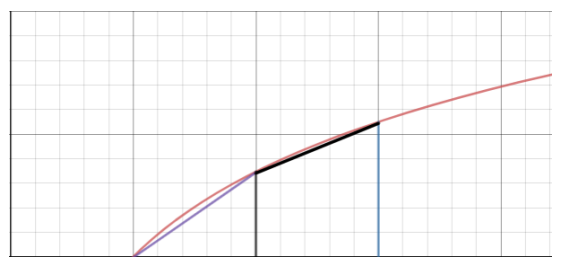
\includegraphics[width=20\baselineskip]{figures/trapezoidal_under.png}\\
Approach one is two use a trapezoid whose bases are at the integers themselves.\\

Area of the trapezoids is $\frac{1}{2}\sum_{i=1}^{n-1}{[ln(i)+ln(i+1)]}$\\
$=\frac{1}{2}ln(1)+\sum_{i=2}^{n-1}{[ln(i)+ln(i+1)]}+\frac{1}{2}ln(n)$\\
$=ln(n!)-\frac{1}{2}ln(n)$\\

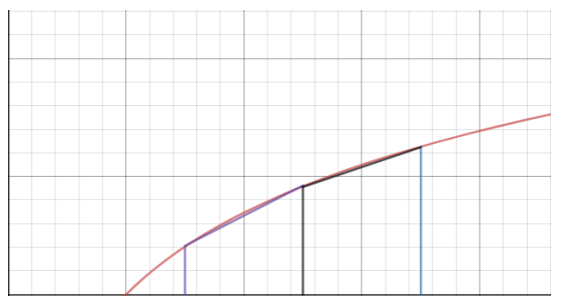
\includegraphics[width=20\baselineskip]{figures/trapezoidal_over.png}\\
Approach two is two use a trapezoid whose bases are at the midpoints between integers. Notice that we don't care about the area before $x=\frac{1}{2}$ in our calculations.\\ 

Area = $ln(2)+ln(3)+ln(4)\dots+ln(n-1)+\frac{1}{2}ln(n)$, which comes out to be the same as above.  Notice that this is an overestimate however, and the previous approach was an underestimate.\\
$\therefore \int_{\frac{3}{2}}^{n}{ln(x)}dx + \frac{1}{2}ln(n) < ln(n!) < \int_{1}^{n}{ln(x)}dx + \frac{1}{2}ln(n)$\\

Given $\int{ln(x)}dx = xln(x) - x + C$\\

We get:\\
$(nln(n)-n)-(\frac{3}{2}ln(\frac{3}{2}) - \frac{3}{2}) + \frac{1}{2}ln(n) < ln(n!) < (nln(n) - n) - (ln(1) - 1) + \frac{1}{2}ln(n)$\\
$=(n+\frac{1}{2})ln(n)-n-\frac{3}{2}(ln(\frac{3}{2}) - 1) < ln(n!) < (n+\frac{1}{2})ln(n) - n + 1$\\

At this point, we have a range of error for $ln(n!)$.\\

We can define $ln(n!) = [(n+\frac{1}{2})ln(n) - n] + \delta_n$, where $\frac{3}{2}(1-ln(\frac{3}{2})) < \delta_n < 1 \longrightarrow 0.891802 < \delta_n < 1$\\

Since $ln(n!) = (n+\frac{1}{2})ln(n) - n + \delta_n$,\\
$e^{ln(n!)} = e^{nln(n)}e^{\frac{1}{2}ln(n)}e^{-n}e^{\delta_n}$\\
$n! = n^n \sqrt(n) e^{-n}e^{\delta_n}$\\
$=(\frac{n}{e})^n \sqrt(n) * e^{\delta_n}$, where $e^{\delta_n} \in [2.439, 2.718]$. The value for $\sqrt{2 \pi n} = 2.506$, which falls within our expected range of values.

\end{proof}

Now that we have an approximation for $n!$, we can look to write an expression that will give us the $n^{th}$ Catalan number. The $n^{th}$ Catalan number is given by the expression $\binom {2n} n*\frac{1}{n+1}$\\
$\binom{2n}n*\frac{1}{n+1} = \frac{(2n)!}{n!n!} = \frac{(2n)!}{[(\frac{n}{e})^n * \sqrt{2\pi n}]^2}$\\
$= \frac{\frac{2n}{e}^{2n}}{\frac{n}{e}^{2n}} * \frac{\sqrt{4\pi n}}{2\pi n * (n+1)} = \frac{2^{2n}*\sqrt{\pi n}}{\pi n(n+1)} = \frac{4^n}{\sqrt{\pi n}(n+1)}$

\subsection{Gamma Function}
Gamma functions are an extension of factorials, such that the arguments are shifted down by one. In other words, $\Gamma(2) = 1!$, $\Gamma(3) = 2!$, etc. We intend to prove that $\Gamma(n+1) = n!$. To do this, we first begin by defining our gamma function.\\
\begin{definition}
    $\Gamma(z+1)=\int_{0}^{\infty} {x^{z}e^{-x}}$
\end{definition}
Now that we have defined our gamma function, we will attempt to prove that $\Gamma(n+1) = n!$.\\
\begin{proof}
First, we will integrate this function by parts:
\begin{multicols}{2}
\begin{itemize}
    \item $u = x^7$, $du = zx^{z-1}$
    \item $v = -e^{-x}$, $dv=e^{-x}$
\end{itemize}
\end{multicols}
$\therefore \int_{0}^{\infty}{x^{z}e^{-x}dx} = [x^{z}(-e^{-x})]_{0}^{\infty} + \int_{0}^{\infty}{zx^{z-1}e^{-x}dx}$\\

Notice how when we evaluate the expression $\int_{0}^{\infty}{x^{z}e^{-x}dx} = [x^{z}(-e^{-x})]_{0}^{\infty}$, $x^{z}$ becomes $0$ when evaluated at $x=0$, and $(-e^{-x})$ becomes zero when evaluated at $x=\infty$, meaning that this expression evaluates to just $0$. \\

Therefore, we are left with just $\int_{0}^{\infty}{zx^{z-1}e^{-x}dx}$. We can redefine this as $z\int_{0}^{\infty}{x^{z-1}e^{-x}dx} = z\Gamma(z)$.\\

At this point, we have something that is similar to a factorial, but we can't consider our proof complete until we establish some base cases. We can begin by testing with $z=1$. $\Gamma(1) = \int_{0}^{\infty}{x^{0}e^{-x}}dx = \int_{0}^{\infty}{e^{-x}}dx = 1$\\
$\therefore \Gamma(1) = 1$\\
$\Gamma(2) = 1 * \Gamma(1) = 1$\\
$\Gamma(3) = 2 * \Gamma(2) = 3$\\
$\Gamma(4) = 3 * \Gamma(3) = 6$\\
$\therefore \Gamma(n+1) = n!$
\end{proof}
As we intended, we have now found a function that is similar to a factorial, withe the arguments shifted by one. However, we also want to observe how fractional factorials work. In our case, we'll observe $\Gamma(\frac{1}{2})$. 
\begin{proof}
$\Gamma(\frac{1}{2})=\int_{0}^{\infty}{x^{\frac{-1}{2}}e^{-x}}dx = \int_{0}^{\infty}{\frac{e^{-x}}{\sqrt{x}}}$\\
Let $u=\sqrt{x}$, $u^2=x$, and $du*2u=dx$\\
Substituting $u$ into the equation, we get $\Gamma(\frac{1}{2})=2\int_{0}^{\infty}{e^{-u^2}}du$\\
Now suppose we define a variables $v$ and $K$, such that\\
$K=\int_{0}^{\infty}{e^{-u^2}}du = \int_{0}^{\infty}{e^{-v^2}}dv$\\
$K^2=\int_{0}^{\infty}{e^{-u^2}}du \int_{0}^{\infty}{e^{-v^2}}dv$\\
$=\int_{0}^{\infty}\int_{0}^{\infty}{e^{-u^2}e^{-v^2}}dudv = \int_{0}^{\infty}\int_{0}^{\infty}{e^{-(u^2+v^2)}}dudv$\\
In Cartesian coordinates, this integral would be difficult to solve. However, we can convert to polar coordinates to solve this equation. Notice that because we are only using positive integers, $\theta$ is bounded within the first quadrant\\
$K^2=\int_{0}^{\frac{\pi}{2}}\int_{0}^{\infty}{e^{-r^2}*r}drd\theta = \frac{\pi}{2}\int_{0}^{\infty}{e^{-r^2}*r}dr$\\
$=\frac{\pi}{2}*(\frac{-e^{-r^2}}{2})_{0}^{\infty} = \frac{\pi}{2}(\frac{1}{2} - 0) = \frac{\pi}{4}$\\
$\therefore K = \frac{\sqrt{\pi}}{2}$\\
$\therefore \Gamma(\frac{1}{2}) = 2K = 2\frac{\sqrt{\pi}}{2} = \sqrt{\pi}$
\end{proof}
% \end{document}
